\section{\label{sec:nmp:pespecific}\texorpdfstring{\Glsentrylong{pe}}{Proxel}-specific asynchronous messaging}
\cpresetrulenumber

This section presents a variant of the above system where the \glspl{pe} run \emph{asynchronously} \cite{Balanescu2011,Nicolescu2014} (the concept of asynchronicity used here is different to that of \cite{Cavaliere2009,Frisco2012,Song2013} and related) so that the steps of one \gls{pe} do not necessarily occur contemporaneously with those of another.  In this form, \gls{nmp} shares some obvious similarities with the Actor model \cite{Agha1986} and Communicating Sequential Processes \cite{Hoare1985}.  

There is no longer a single state spanning the entire system.  Instead, each \gls{pe} has its own state dictating its operation individually.  The same conceptual phases are kept, though the \gls{oq} and \gls{nm} phases are combined because they now may occur interleaved.  During the \gls{oq} \& \gls{nm} phase, each \gls{pe} independently works through a series of \emph{rounds}, following the typical idea of a round in theoretical asynchronous systems:  The \gls{pe} receives one or more messages, processes the received messages and updates its internal data, then sends out new messages based on the results.

The most significant change from \cref{sec:nmp:systemwide} is perhaps the use of \emph{receipt tokens}.  Receipt tokens show that the \gls{pe} has received a message from a particular neighbour since the last time messages were sent.  This is vital to ensure that the correct number of messages are sent, and sent only after receiving appropriate messages from other neighbours.  Initialisation of the \glspl{pe} differs slightly from \cref{sec:nmp:systemwide}.  Along with the channels, each \gls{pe} also starts with an adjacency list object, \(\cpfunc{a}{A}\), which holds a copy of the atoms for each neighbour/channel.

\begin{figure}
    \centering
    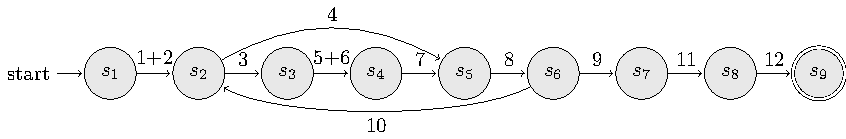
\includegraphics[width=1.0\textwidth]{chapters/nmp/images/proxelspecificstatemachine.pdf}
    \caption[State machine of the progression of the \acrshort{pe}-specific \acrlong{nmp} \gls{cps} rules]{State machine of the progression of the \gls{pe}-specific \gls{nmp} \gls{cps} rules.  The vertices are labelled with the states and the arcs with the rule(s) which cause that transition.}
    \label{fig:nmp:proxelspecificstatemachine}
\end{figure}

As with \cref{sec:nmp:systemwide}, we show the progression of the system through its states in \cref{fig:nmp:proxelspecificstatemachine}.  In this system, an \gls{oq} \& \gls{nm} round can be regarded as the steps taken to proceed from state \(s_2\) until reaching \(s_2\) again.  Thus, receiving one or more messages, followed potentially by preparing and sending new messages, forms a round.  The initialisation phase is only rules 1 and 2.  The combined \gls{oq} and \gls{nm} phase is made up of rules 3 through 10, which involve the receipt of one or more messages with generation \(0 < g \leq I\) from neighbours, then preparation of new messages to send to neighbours through communicating with the oracle and forwarding the results of the oracle's computation to the relevant neighbours.  Lastly, rules 11 and 12 make up the finalisation phase.

\begin{algorithm}
\DontPrintSemicolon
\SetKwFunction{Uniq}{uniq}
\SetKwFunction{Perm}{permutations}
\SetKwFor{pForEach}{parallel foreach}{do}{endfch}
\SetKwBlock{Loop}{loop:}{}
\SetKw{KwOr}{or}
\SetKw{KwAnd}{and}
\SetKw{KwGoto}{goto}
\KwIn{Adjacency set \(A = \{1,2,3,4\}\)}
\KwOut{Final result, \(z\), sent to \(e\)}
\Begin{
    \tcc{
    \(a \Leftarrow \langle b \rangle\) denotes receiving object \(a\) on channel \(b\)\newline
    \(c \Rightarrow \langle d \rangle\) denotes sending object \(c\) on channel \(d\)
    }\;
    
    \tcc{Initialisation}
    \(R \gets \emptyset\)\;
    \(i \Leftarrow \langle e \rangle\)\;
    
    \tcc*[l]{* assume environment \(e\) sends all of these}
    \pForEach{\((x, 0, d) \Leftarrow \langle e \rangle\)}{
        \(v[x] \gets (0,d)\)\;
        \(R \gets R \cup \{x\}\)
    }
    
    \;\tcc{\Glsentrylong{oq} \emph{and} \Glsentrylong{nm}}
    
    \Loop{
        \(W \gets \emptyset\)\;
        
        \pForEach{\((x,y,z,w) \in\) \Perm{\(A\)}}{
            \If{\(x \in R\) \KwAnd \(v[x].g < i\) \KwAnd \(v[x].g \leq v[y].g\) \KwAnd \(v[x].g \leq v[z].g\)}{
                \(W \gets W \cup (w,v[x].g+1, v[x].d \cup v[y].d \cup v[z].d))\)\label{line:nmp:rule3}
            }
        }
        
        \If{\(W \not= \emptyset\)}{
            \(W \gets\) \Uniq{\(W\)} \tcc*[l]{Multiset to set}
            \;
            \lpForEach{\((w, g, d) \in W\)}{\((w, g, d) \Rightarrow \langle o \rangle\)}
            \tcc*[l]{** assume oracle \(o\) returns all required messages}
            
            \lpForEach{\((w, g, d) \Leftarrow \langle o \rangle\)}{\((w, g, d) \Rightarrow \langle w \rangle\)}
            \(W \gets \emptyset\)
        }
        
        \(R \gets \emptyset\)\;
        \;
        \(b \gets\) \texttt{true}
        
        \lpForEach{\(x \in A\)}{\lIf*{\(v[x].g < i\)}{\(b \gets\) \texttt{false}}}
        \lIf{b}{\KwGoto break}\;
        
        \While{\(|R| = 0\)}{\label{line:nmp:recvwhile}
            \pForEach{\((x, g, d) \Leftarrow A\)}{\label{line:nmp:recvfor}
                \(v[x] \gets (g,d)\)\;
                \(R \gets R \cup \{x\}\)\;
            }
        }
        \KwGoto loop\;
    }
    \AlCapSty{\AlCapFnt break:}\;
    
    \;\tcc{Finalisation}
    
    \lpForEach{\(x \in A\)}{\(v[x] \Rightarrow \langle o \rangle\)}
    \(z \Leftarrow \langle o \rangle\)\;
    \(z \Rightarrow \langle e \rangle\)
}
\caption[Pseudocode description of the process for an individual \gls{fne} \acrshort{pe} in the asynchronous system]{\label{alg:nmp:pespecific}Pseudocode description of the process for an individual \gls{fne} \gls{pe} in the asynchronous system}
\end{algorithm}

Again, we also supply a pseudocode representation of the procedure in \cref{alg:nmp:pespecific}.  The pseudocode does not closely resemble the ruleset of \cref{ruleset:nmp:proxspec} in appearance.  Instead, the pseudocode is written to reflect best the meaning and intention of the rules while still relating it to the ruleset.

An important assumption for this ruleset is that the oracle returns all outstanding results together.  After a \gls{pe} sends one or more \gls{oq} messages to the oracle, it enters a blocking wait until it receives updated \gls{nm} messages back from the oracle.  One \gls{nm} message is expected per \gls{oq} message.  We assume that the oracle returns all these messages during one step, possibly waiting until it has finished computing new values for every message.  We make the same assumption for finalisation, and similarly, assume that the environment sends in all the initial messages during a single step.

In preparing the new \gls{oq} messages to go to the oracle, rule 3 discards the information about which datum came from which neighbour (visible in line \ref{line:nmp:rule3} in \cref{alg:nmp:pespecific}).  This is irrelevant for \gls{bp} \gls{sm}.  It might be relevant, however, to keep said information for a different computation.  One must bear this in mind when adapting the rules to their problem.  The changes needed are likely minor, but we do not explore them further as they are superfluous.

\subsection{System Definition}
Per the tuple definition from \cref{sec:cps:formaldescriptions}:

\(T\) is a set of top-level cells, each representing a single \gls{pe}, numbered sequentially.  These numbers correspond to the \(\iota\) of \cref{fig:nmp:iota_proxels_environment_oracle}.  \(A\) is equal to the set of terms defined in \cref{sec:pespecific:definitions}.  Each \gls{pe}'s starting multiset in \(O\) is the appropriate channel endpoints and an adjacency list term \(a\).  Every \gls{pe}'s ruleset in \(R\) is either equal to that found in \cref{ruleset:nmp:proxspec}, or one which starts with that ruleset as a base.  These latter rulesets drop terms from rule 3 to adapt it to the relevant \gls{pe} having fewer than four neighbours (see \cref{sec:nmp:ruleslessthanfour}).  \(S = \{s_1, \dots, s_9\}\) and \(\bar{s} = s_1\).

\subsection{Description of Rules}

\begin{cprulesetfloat}
    \begin{cpruleset}
    
        %%%%%%%%%%%%%  Initialisation  %%%%%%%%%%%%%
    
        % Receive inputs from environment
        \cprule{s_1}{\cprecv{\cpfunc{i}{I}}{e}}{1}{s_2}{\cpfunc{i}{I}}
        
        \cprule{s_1}{\cprecv{\cpvv{X}{\cpempty}{D}}{e}}{+}{s_2}{\cpvv{X}{\cpempty}{D} & \\ & & & & \cpfunc{r}{X}}
        
        \\
        
        %%%%%%%%%%%%%  OQ & MP phase  %%%%%%%%%%%%%
        
        \cprule{s_2}{}{+}{s_3}{\cpvw{W}{G\cpundig}{\cpfunc{d}{A}\,\cpfunc{d}{B}\,\cpfunc{d}{C}}}
        \cppromoter{\cpfunc{r}{X}}
        \cppromoter{\cpvv{X}{G}{A}}
        \cppromoter{\cpvv{Y}{G\_}{B}}
        \cppromoter{\cpvv{Z}{G\_}{C}}
        \cppromoter{\cpfunc{i}{G\cpundig\_}}
        \cppromoter{\cpfunc{a}{\cpfunc{n}{X}\,\cpfunc{n}{Y}\,\cpfunc{n}{Z}\,\cpfunc{n}{W}}}
        
        \cprule{s_2}{}{1}{s_5}{}
        
        \cprule{s_3}{\cpvw{W}{\_}{\_}}{+}{s_4}{}
        \cppromoter{\cpvw{W}{\_}{\_}}
        
        % Send to oracle
        \cprule{s_3}{\cpvw{W}{G}{D}}{+}{s_4}{\cpsend{\cpvw{W}{G}{D}}{o}}
        
        % Receive from oracle & send to neighbour
        \cprule{s_4}{\cprecv{\cpvw{W}{G}{D}}{o}}{+}{s_5}{\cpsend{\cpvv{W}{G}{D}}{W}}
        
        % Clear all receipt tokens at the end of a send process
        \cprule{s_5}{\cpfunc{r}{\_}}{+}{s_6}{}
        
        % Transition to end if all generations complete
        \cprule{s_6}{}{1}{s_7}{}
        \cpinhibitor{\cpvv{X}{G}{D}}
        \cppromoter{\cpfunc{i}{G\cpundig\_}}
        
        %receive messages
        \cprule{s_6}{\cprecv{\cpvv{\_}{G\cpundig}{D}}{X} & & & \\ & \cpvv{X}{G}{\_}}{+}{s_2}{\cpvv{X}{G\cpundig}{D} &\\ & & & & \cpfunc{r}{X}}
        
        \\
        
        %%%%%%%%%%%%%  Finalisation %%%%%%%%%%%%%
        
        % Send to oracle
        \cprule{s_7}{\cpvv{X}{G}{D}}{+}{s_8}{\cpsend{w'\perfectunary{IncreaseHeight}{(}{)}{X}\perfectunary{IncreaseHeight}{(}{)}{G}\perfectunary{IncreaseHeight}{(}{)}{D}}{o}}
        
        % Oracle returns results which are immediately emitted to the environment
        \cprule{s_8}{\cprecv{\cpfunc{z}{Z}}{o}}{\cpundig}{s_9}{\cpsend{\cpfunc{z}{Z}}{e}}
        
    \end{cpruleset}
    \caption[Ruleset for the \gls{fne} \acrshort{pe}-specific asynchronous \acrlong{nmp} system, for an inner \acrshort{pe}]{\label{ruleset:nmp:proxspec}Ruleset for the \gls{fne} \gls{pe}-specific asynchronous \gls{nmp} system, for an inner \gls{pe} (i.e., one not on the border) and using an oracle to compute the data for outgoing messages}
\end{cprulesetfloat}

\begin{enumerate}
    \item Receive the \(\cpfunc{i}{I}\) input from the environment.
    \item Receive \(\cpvv{X}{\cpempty}{D}\) messages as inputs from the environment.
    \item Consider in turn all receipt tokens \(r\), if any (in any arbitrary order). For \(\cpfunc{r}{k_1}\) and \(\cpvv{k_1}{g_1}{\_}\), compare generation number \(g_1\) against the generation numbers of all other current values \(\cpvv{k_j}{g_j}{\_}, k_j \in \{k_2, k_3, k_4\} = \{1, 2, 3, 4\} \setminus \{k_1\}\). Without loss of generality, if \(g_1 \leq g_2, g_3\) \emph{and} \(g_1 < I\) (i.e., the maximum generation count) then create a message \(w\) to send to the oracle for \gls{oq}.  This message has the data for \(k_1\), \(k_2\) and \(k_3\), which are used by the oracle in computing the new message to send to \(k_4\).  The generation count for this \(w\) message is \(g_1 + 1\).
    \item If there were no \gls{oq} messages generated by rule 3, then move straight to the process of testing for termination and receiving new messages.
    \item If rule 3 resulted in the creation of more than one \gls{oq} message about a given neighbour, select one of those messages at random and delete the others.  The messages will be identical, but duplicates may arise due to the unification of different neighbours to \(Y\) and \(Z\) in rule 3.
    \item For each \gls{oq} message remaining after rule 5, send said message to the oracle to compute the new corresponding outgoing \gls{nm} message.
    \item Forward newly prepared \gls{nm} messages \(v\) from the oracle to the relevant neighbour.
    \item Delete all extant receipt tokens after completing the relevant \gls{oq} \& \gls{nm} phase.
    \item If messages with a generation count equal to \(I\) have been received from every neighbour, transition to the finalisation phase.
    \item Receive a message \(\cpvv{\_}{G}{D}\) from neighbour \(X\) and replace the current \(v\) object for \(X\) with it.  The neighbour label contained inside the message is overwritten with the current \gls{pe}'s label for the receiving channel.  Create a receipt token \(\cpfunc{r}{X}\).
    \item Send all the \gls{pe}'s \(v\) messages to the oracle, for the oracle to compute the final output for the \gls{pe}.
    \item Receive the computed final result from the oracle and send it to the environment.
\end{enumerate}

\subsection{\label{sec:pespecific:definitions}Definitions of Terms}

\paragraph{Atoms}
The same as in \cref{sec:nmp:systemwide}.

\paragraph{Functors}
\begin{description}
    \cptermdef{a}{Adjacency set.  Lists the neighbours of the \gls{pe} as a set of \(n\) functors.}
    \cptermdef{i}{Maximum generations counter.  Used slightly differently to \cref{sec:nmp:systemwide}.}
    \cptermdef{n}{Neighbourhood functor.  Stores the label for one of the channels/neighbours to which the current \gls{pe} is connected.}
    \cptermdef{r}{Receipt token, showing that a message was recently received from neighbour \(X\).}
    \cptermdef{v}{Serves as both the internal data stores and \gls{nm} messages of the system.  These are the \(v\) compound terms described in \cref{sec:cps:compoundterms}.}
    \cptermdef{w}{Identical in most respects to \(v\) functors, except used for messaging with the oracle instead of neighbouring \gls{pe}.  That is, these are \gls{oq}, rather than \gls{nm}, messages.}
    \cptermdef{w'}{Identical to \(w\), except marked to indicate to the oracle that the messages sent are to be used for finalisation computations instead of \gls{oq}.}
    \cptermdef{z}{Identical to the \(z\) in \cref{sec:nmp:systemwide}.}
\end{description}

\paragraph{States}
\begin{description}
    \cptermdef{s_1}{Environmental inputs receipt state.}
    \cptermdef{s_2}{Messaging round starting state.  If it is appropriate for the \gls{pe} to send new messages to its neighbours, then \gls{oq} messages are prepared and the sending process continues.  Otherwise, return to receiving once again.}
    \cptermdef{s_3}{Message send phase, part 1.  Drop any duplicate \gls{oq} messages referring to the same neighbour.   Send \gls{oq} messages to compute new outgoing \gls{nm} messages.}
    \cptermdef{s_4}{Receive the new \gls{nm} messages computed by the oracle, and forward them to the appropriate neighbour(s).}
    \cptermdef{s_5}{Receipt token deletion state.  Unconditionally delete all receipt tokens present.}
    \cptermdef{s_6}{Message receipt state.  When there are no messages to send, the \gls{pe} performs a `blocking' receipt (see \cref{sec:cps:blocking}) in this state until one or more of its neighbours send messages on the connecting channels.}
    \cptermdef{s_7}{Equivalent to state \(s_5\) in \cref{sec:nmp:systemwide}.}
    \cptermdef{s_8}{Equivalent to state \(s_6\) in \cref{sec:nmp:systemwide}.}
    \cptermdef{s_9}{Equivalent to state \(s_7\) in \cref{sec:nmp:systemwide}.}
\end{description}

% \subsection{\label{sec:nmp:ruleslessthanfour}Rules for \texorpdfstring{\gls{fne}}{four-neighbourhood} \texorpdfstring{\acrshort{pe}s}{proxels} with fewer than four neighbours}
\subsection{\label{sec:nmp:ruleslessthanfour}Rules for \glsentrytext{fne} \glsentrytext{pe}s with fewer than four neighbours}

The rules of \cref{ruleset:nmp:proxspec} consider only the case where a \gls{pe} has exactly four neighbours.  These would not work correctly for those \glspl{pe} with three neighbours (i.e., on the grid border, but not in a corner) or two neighbours (i.e., in a grid corner).  The only adjustment necessary to handle these edge cases is to change the number of neighbours considered, specifically in rule 3.

These alternative rules are listed in \cref{ruleset:nmp:3alts} as rule 3a and rule 3b for the border and corner cases, respectively.  We assume henceforth that any \gls{nmp} system is constructed to handle the finite boundaries of the grid correctly by replacing the usual rule 3 with the suitable alternative for edge \glspl{pe}.  \cref{sec:nmp:example} uses rule 3a to simplify and shorten the example without neglecting the essential details.

\begin{cprulesetfloat}
    \begin{cpruleset}
        \cprulecustnum{s_2}{}{+}{s_3}{\cpvw{W}{G\cpundig}{\cpfunc{d}{A}\,\cpfunc{d}{B}}}{3a}
        \cppromoter{\cpfunc{r}{X}}
        \cppromoter{\cpvv{X}{G}{A}}
        \cppromoter{\cpvv{Y}{G\_}{B}}
        \cppromoter{\cpfunc{i}{G\cpundig\_}}
        \cppromoter{\cpfunc{a}{\cpfunc{n}{X}\,\cpfunc{n}{Y}\,\cpfunc{n}{W}}}
        
        \\
        
        \cprulecustnum{s_2}{}{+}{s_3}{\cpvw{W}{G\cpundig}{\cpfunc{d}{A}}}{3b}
        \cppromoter{\cpfunc{r}{X}}
        \cppromoter{\cpvv{X}{G}{A}}
        \cppromoter{\cpfunc{i}{G\cpundig\_}}
        \cppromoter{\cpfunc{a}{\cpfunc{n}{X}\,\cpfunc{n}{W}}}
        
    \end{cpruleset}
    \caption[Alternative forms of \cref{ruleset:nmp:proxspec}'s rule 3]{\label{ruleset:nmp:3alts}Alternative forms of \cref{ruleset:nmp:proxspec}'s rule 3 for \glspl{pe} on the border of a grid or in the corner of a grid, respectively}
\end{cprulesetfloat}

A strength of \gls{cps} in earlier work has been the fact that one rule system applies to all possible problems \cite{Cooper2019a,Cooper2019}.  Modifying the rules to fit the problem weakens that strength.  An alternative is the use of `dummy' or `sentinel' \glspl{pe} with special rules outside the grid connected to the corner and border \glspl{pe}.  The specifics of the special rules are situation-dependent and so unexplored here.

\subsection{Traces}

A \emph{trace} is a sequence of \emph{snapshots}, connected by arrows \tarr{}, describing the evolution of message generation numbers. A snapshot is an \(m\)-tuple, where \(m\) is the number of neighbours for the relevant \gls{pe}:  \((g_1, g_2, g_3, g_4)\) for a \gls{fne}, where \(g_k\) is the generation number of the last message \(\cpvv{k}{g_k}{\_}\) received from neighbour \(k\).  The period between snapshots is a \emph{round}, as described above.  The initialisation and finalisation phases may be included in a trace as single rounds along with \gls{oq} \& \gls{nm}.

By convention, for a \gls{fne} \gls{pe}, the entries in a snapshot are written clockwise starting from the top.  That is, the first entry is the neighbour above the current \gls{pe}, the second entry the neighbour to the right, \textit{et cetera}.  If there is no message pertaining to a given neighbour present inside the relevant \gls{pe}/top-level cell, `--' is used in place of the corresponding generation number.

Optionally, snapshots may be decorated further with 
{\renewcommand{\theenumi}{\alph{enumi}}
\begin{enumerate}
    \item A round number, \(h\): \trace{\(g_1\)}{\(g_2\)}{\(g_3\)}{\(g_4\)}\(_h\).
    \item Each component \(g_k\) can be followed by a question mark \(?\), showing that a message was just received from that neighbour at the start of the current round.
    \item Each component \(g_k?\) can be further followed by one or more stars \(*\), one for each message sent because of the corresponding incoming message.
\end{enumerate}}

Contemporaneous receipts from different neighbours may lead to the same outgoing message(s).  As a convention, the left-most \(g_k?\) which triggers the outgoing message will be marked with the corresponding \(*\).

For example, a snapshot where the latest iterations received from the first through fourth neighbours are 2, 3, 1 and 2, respectively, and a message has just been received from neighbour four, would look like:  \trace{2}{3}{1}{2?*}.  A trace documenting this could look like \tracen{2}{3}{1}{1} \tarr{} \tracen{2}{3}{1}{2?*}.